\documentclass[../DoAn.tex]{subfiles}
\usepackage{xcolor}
\usepackage{float}
\usepackage{needspace}

\newcommand{\UCtitle}[1]{%
    \needspace{12\baselineskip}
    \vspace{1em}
    {\large\bfseries #1}\\[-0.5em]
    \rule{\textwidth}{0.5pt}
}

\begin{document}

% ============================================================
\section{Khảo sát hiện trạng và vấn đề tồn tại}

\subsection{Hiện trạng hệ thống}

Hiện nay, nhiều nhà hàng vẫn vận hành theo phương thức quản lý thủ công hoặc sử dụng các công cụ rời rạc như sổ ghi chép, Excel hoặc trao đổi trực tiếp giữa các bộ phận. Thông tin đặt bàn của khách hàng thường được tiếp nhận qua điện thoại hoặc mạng xã hội và ghi lại thủ công, dẫn đến dữ liệu phân tán và không được đồng bộ giữa các nhân viên.

Trong quá trình phục vụ, nhân viên thường ghi order bằng giấy rồi chuyển cho bếp, trong khi việc cập nhật trạng thái món ăn chủ yếu dựa vào trao đổi trực tiếp. Bên cạnh đó, hoạt động theo dõi doanh thu thường được thực hiện thông qua bảng tính hoặc tổng hợp thủ công, chưa có sự liên kết với các hoạt động vận hành khác.

Nhìn chung, hệ thống hiện tại thiếu một nền tảng quản lý tập trung, các quy trình nghiệp vụ hoạt động rời rạc và phụ thuộc nhiều vào thao tác thủ công.

\subsection{Vấn đề tồn tại}

Từ thực trạng trên, có thể thấy hệ thống quản lý nhà hàng hiện tại còn tồn tại nhiều hạn chế. Trước hết, việc phụ thuộc vào ghi chép thủ công trong các quy trình như đặt bàn và ghi nhận đơn hàng dễ dẫn đến các sai sót như trùng lịch đặt bàn, thất lạc thông tin hoặc nhầm lẫn món ăn.

Ngoài ra, dữ liệu trong hệ thống không được cập nhật theo thời gian thực, gây khó khăn cho nhà quản lý trong việc theo dõi tình trạng hoạt động và kiểm soát doanh thu. Hệ thống hiện tại cũng chưa cung cấp một nền tảng trực tuyến để khách hàng có thể xem menu, đặt bàn hoặc theo dõi trạng thái phục vụ, làm giảm trải nghiệm người dùng. Đồng thời, việc thiếu các công cụ báo cáo và thống kê trực quan khiến quá trình đánh giá hiệu quả kinh doanh và đưa ra quyết định quản lý trở nên kém hiệu quả.

\section{Xác định tác nhân}

Hệ thống có các nhóm người dùng chính gồm khách hàng, nhân viên phục vụ, nhân viên bếp, quản lý chi nhánh và quản trị hệ thống; mỗi nhóm đảm nhận các vai trò khác nhau trong quá trình vận hành và quản lý nhà hàng. Hệ thống phân quyền theo vai trò để giới hạn chức năng truy cập.

% ============================================================
\section{Yêu cầu chức năng}
% ============================================================

Phần này mô tả các nhóm chức năng chính của hệ thống, được tổng hợp từ các Use Case UC01--UC17.

\subsection{Chức năng chung}

\begin{itemize}
    \item Đăng nhập hệ thống (UC02).
\end{itemize}

\subsection{Nhóm chức năng dành cho khách hàng}

\begin{itemize}
    \item Đăng ký tài khoản (UC01).
    \item Xem thông tin các chi nhánh; tìm chi nhánh gần vị trí (UC03).
    \item Xem menu món ăn của chi nhánh (UC04).
    \item Đặt bàn trước; tùy chọn đặt món trước sau khi đặt bàn (UC05, UC07).
    \item Xem lịch sử đặt bàn và hóa đơn; theo dõi phiên bàn, gửi yêu cầu thanh toán, hủy đặt bàn khi được phép (UC12).
    \item Gửi đánh giá chất lượng dịch vụ (UC13).
\end{itemize}

\subsection{Nhóm chức năng vận hành tại nhà hàng (Nhân viên phục vụ)}

\begin{itemize}
    \item Tiếp nhận khách và phân bàn (UC06).
    \item Tạo order món ăn cho bàn (UC07).
    \item Phục vụ món ăn cho bàn (UC09).
    \item Cập nhật trạng thái bàn (UC10).
    \item Thanh toán, tạo mã VietQR và xuất hóa đơn cho bàn (UC11).
\end{itemize}

\subsection{Nhóm chức năng bộ phận bếp}

\begin{itemize}
    \item Cập nhật trạng thái chế biến món ăn (UC08).
\end{itemize}

\subsection{Nhóm chức năng quản lý chi nhánh}

\begin{itemize}
    \item Xem báo cáo doanh thu chi nhánh; thống kê đánh giá (UC14).
    \item Quản lý thông tin chi nhánh được giao; quản lý thực đơn chi nhánh (UC15).
\end{itemize}

\subsection{Nhóm chức năng quản trị toàn hệ thống (System Admin)}

\begin{itemize}
    \item Dashboard tổng quan; quản lý các chi nhánh (UC16).
    \item Quản lý nhân viên, tài khoản khách, bàn và phân quyền (UC17).
\end{itemize}

% ============================================================
\section{Yêu cầu phi chức năng}
% ============================================================

Hệ thống quản lý nhà hàng cần đảm bảo các yêu cầu về hiệu năng, độ tin cậy, bảo mật và khả năng mở rộng nhằm đáp ứng nhu cầu vận hành thực tế của một chuỗi nhà hàng nhiều chi nhánh.

\subsection{Hiệu năng và độ tin cậy}
Hệ thống phải đảm bảo thời gian phản hồi nhanh, dưới 1 giây đối với các thao tác phổ biến như xem menu, danh sách bàn và đơn hàng. Các dữ liệu quan trọng cần được xử lý và hiển thị gần như tức thời (khoảng 0,5 giây) nhằm đảm bảo trải nghiệm người dùng mượt mà. Đồng thời, hệ thống phải có khả năng phục vụ từ 50 đến 100 người dùng đồng thời mà không làm suy giảm hiệu năng.

Về độ tin cậy, toàn bộ dữ liệu cần được đảm bảo tính toàn vẹn thông qua cơ chế transaction trong cơ sở dữ liệu (ví dụ gán bàn khi đặt chỗ). Hệ thống cần có cơ chế sao lưu định kỳ và khả năng khôi phục khi xảy ra sự cố. Trạng thái bàn, đơn hàng và món ăn được đồng bộ theo thời gian thực giữa bếp và phục vụ.

\subsection{Bảo mật và quản lý truy cập}
Hệ thống phải đảm bảo an toàn thông tin thông qua việc mã hóa mật khẩu. Cơ chế xác thực và phân quyền theo vai trò giới hạn quyền truy cập chức năng và dữ liệu.

Bên cạnh đó, hệ thống triển khai CAPTCHA khi đăng ký và đặt bàn, giới hạn tần suất thao tác đăng nhập/đặt bàn, và các biện pháp phòng chống SQL Injection, XSS. Tài khoản bị khóa hoặc vô hiệu hóa sẽ bị từ chối đăng nhập.

\subsection{Khả năng mở rộng và vận hành hệ thống}
Hệ thống được thiết kế theo hướng module hóa, cho phép dễ dàng mở rộng số lượng chi nhánh, người dùng và dữ liệu trong tương lai. Các chức năng như quản lý menu, bàn, đơn hàng được tách biệt nhằm hỗ trợ nâng cấp và bảo trì hiệu quả.

Giao diện người dùng cần đảm bảo trực quan, dễ sử dụng và tương thích trên nhiều thiết bị cũng như trình duyệt khác nhau. Ngoài ra, hệ thống phải hỗ trợ theo dõi trạng thái bàn, món ăn và đơn hàng theo thời gian thực để nâng cao trải nghiệm sử dụng.

Về mặt kỹ thuật, hệ thống đảm bảo khả năng triển khai linh hoạt trên môi trường web.

% ============================================================
\section{Kiến trúc phần mềm theo tầng}

Hệ thống backend được tổ chức theo kiến trúc phân tầng gồm năm lớp: \textit{presentation} (controller), \textit{application} (service), \textit{domain} (entity), \textit{infrastructure} (Sequelize, WebSocket) và \textit{crosscutting} (JWT, validation, phân quyền). Các tầng trên chỉ phụ thuộc xuống các tầng dưới, không phụ thuộc ngược.

\begin{figure}[H]
    \centering
    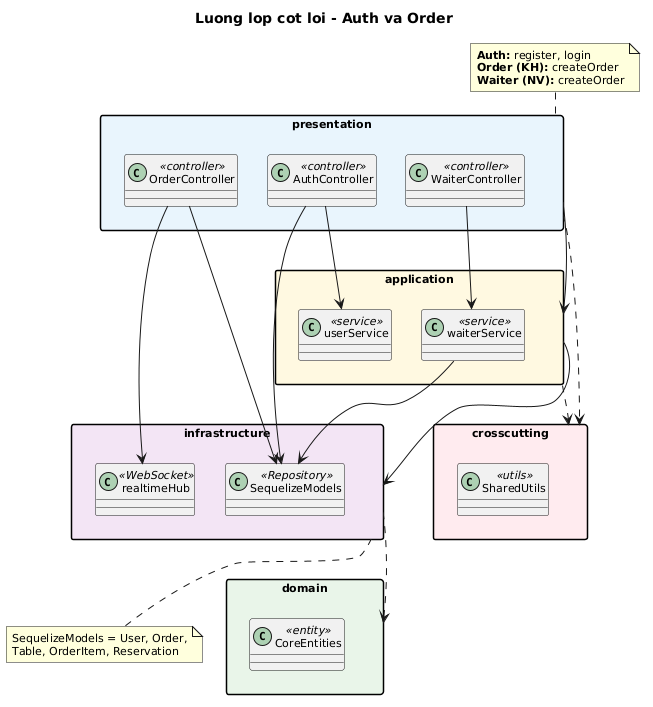
\includegraphics[width=\textwidth,keepaspectratio]{diagrams/class-diagram-core-flow.png}
    \caption{Biểu đồ lớp cốt lõi --- luồng xác thực và đơn hàng}
    \label{fig:class-diagram-core}
\end{figure}

Hình~\ref{fig:class-diagram-core} mô tả luồng nghiệp vụ chính theo bố cục dọc: request đi từ \textit{presentation} xuống \textit{application}/\textit{infrastructure}, rồi map sang \textit{domain}; \textit{crosscutting} được dùng xuyên tầng.

\begin{figure}[H]
    \centering
    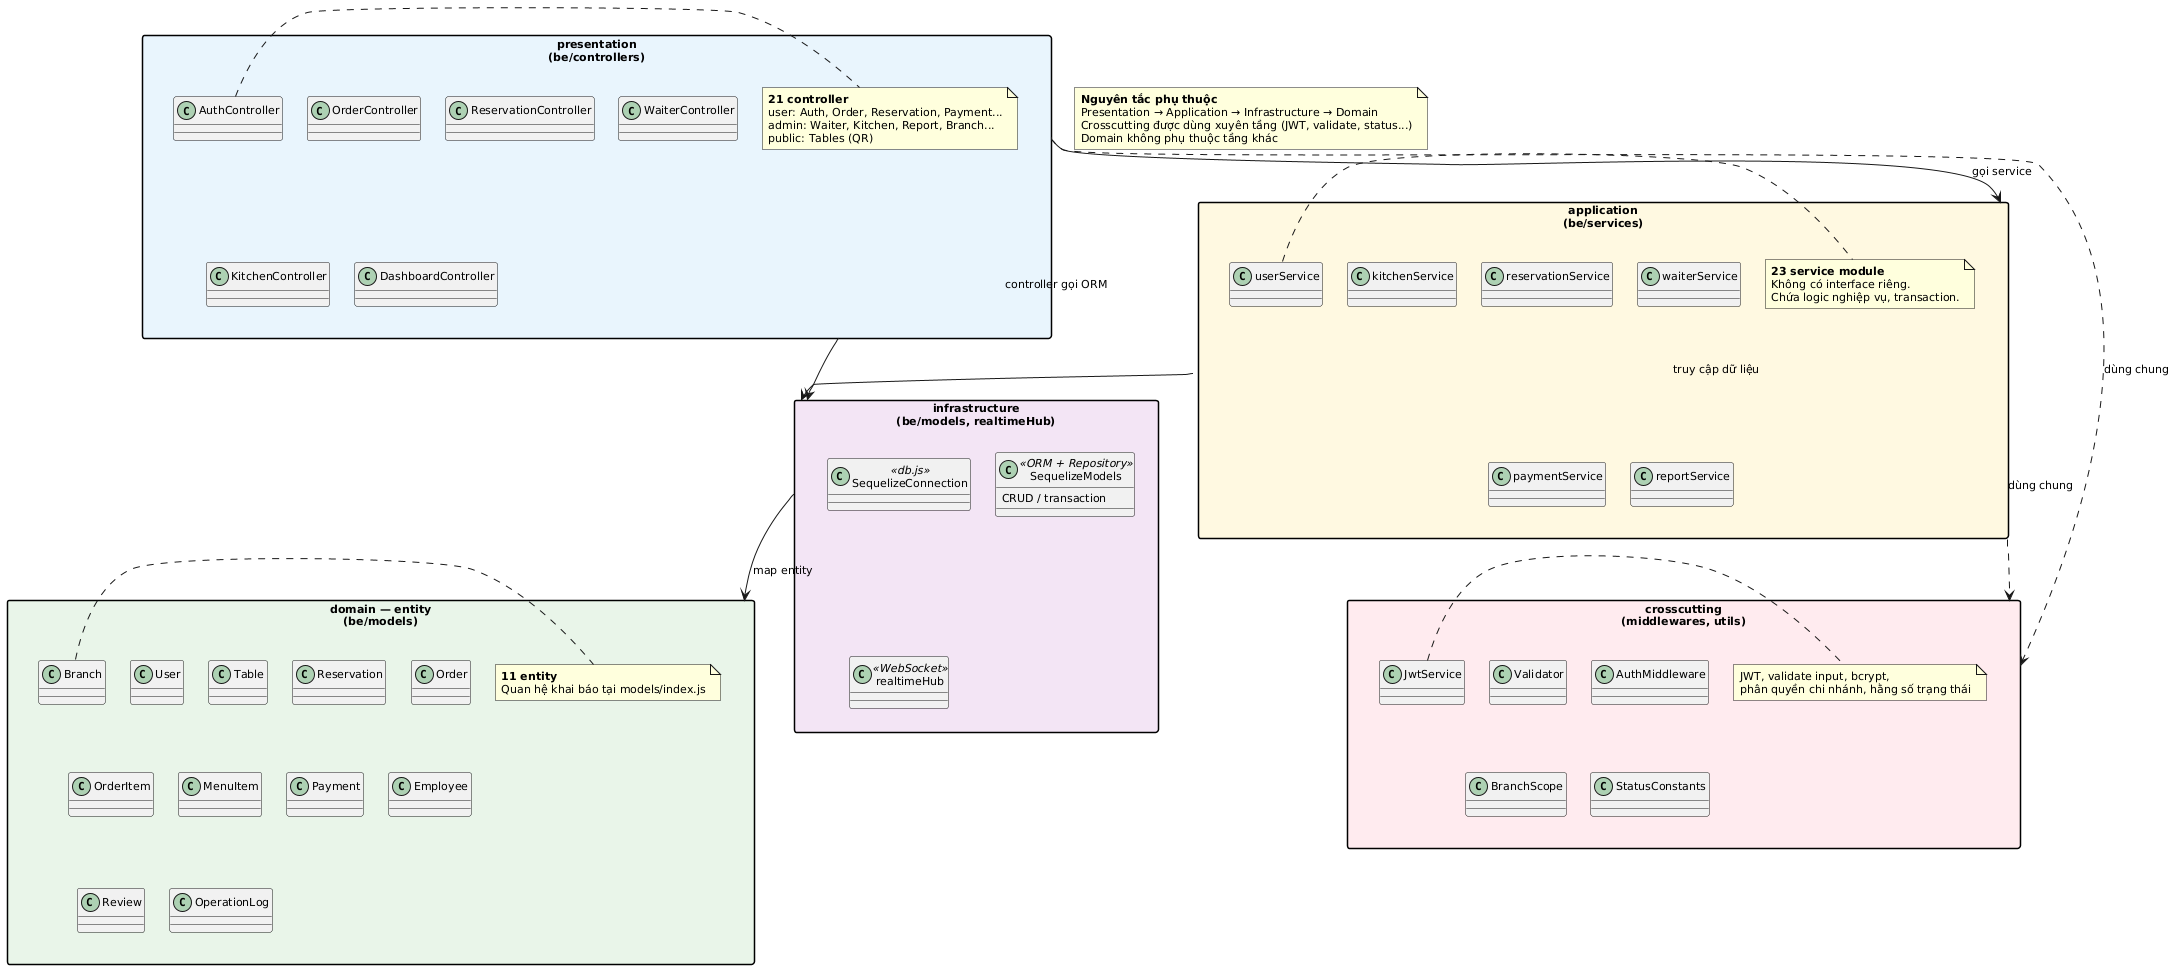
\includegraphics[width=0.85\textwidth,keepaspectratio]{diagrams/class-diagram-layered.png}
    \caption{Biểu đồ tổng quan kiến trúc phân tầng}
    \label{fig:class-diagram-layered}
\end{figure}

Hình~\ref{fig:class-diagram-layered} trình bày tổng quan năm tầng với các thành phần đại diện; chi tiết đầy đủ gồm 21 controller, 23 service và 11 entity.

\begin{figure}[H]
    \centering
    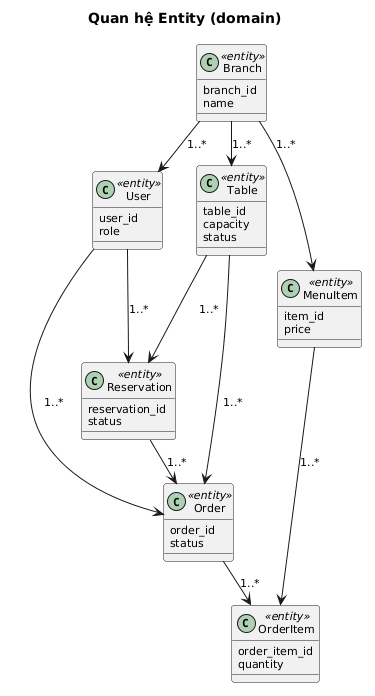
\includegraphics[width=0.75\textwidth,keepaspectratio]{diagrams/class-diagram-domain-entity.png}
    \caption{Biểu đồ quan hệ entity trong tầng domain}
    \label{fig:class-diagram-entity}
\end{figure}

Hình~\ref{fig:class-diagram-entity} mô tả quan hệ giữa các entity cốt lõi, tách riêng khỏi biểu đồ luồng để tránh chồng chéo đường nối.

% ============================================================
\section{Xác định Use Case}
\begin{figure}[htbp]
    \centering
    \includegraphics[width=\textwidth,height=0.8\textheight,keepaspectratio]{Chuong/BDHDKH.png}
    \caption{Biểu đồ hoạt động về quy trình sử dụng dịch vụ của khách hàng}
\end{figure}

\begin{figure}[H]
    \centering
    \includegraphics[angle=-90,width=0.9\textwidth]{Chuong/BDUC.png}
    \caption{Biểu đồ use case tổng quát của hệ thống}
\end{figure}

\UCtitle{UC01 – Đăng ký tài khoản khách hàng}
\begin{table}[H]
\centering
\begin{tabular}{|p{4cm}|p{10cm}|}
\hline
\textbf{Tên Use Case} & Đăng ký tài khoản khách hàng \\ \hline
\textbf{Tác nhân chính} & Khách hàng \\ \hline
\textbf{Tác nhân phụ} & Không có \\ \hline
\textbf{Mục tiêu} &
Khách hàng tạo tài khoản mới bằng cách cung cấp thông tin cá nhân; hệ thống kiểm tra hợp lệ và tạo tài khoản tương ứng.
\\ \hline
\textbf{Điều kiện tiên quyết} &
Khách hàng chưa có tài khoản trên hệ thống và truy cập được vào trang đăng ký.
\\ \hline
\textbf{Điều kiện hậu} &
Tài khoản được tạo thành công và hệ thống thông báo kết quả cho khách. Nếu đăng ký thất bại, hệ thống hiển thị lý do cụ thể.
\\ \hline
\textbf{Luồng sự kiện chính} &
1. Khách hàng nhập thông tin: tên đăng nhập, họ tên, số điện thoại, mật khẩu và xác nhận mật khẩu. \newline
2. Khách hàng hoàn thành CAPTCHA. \newline
3. Hệ thống kiểm tra tính hợp lệ: tên đăng nhập chưa tồn tại; số điện thoại đúng định dạng (10 chữ số, bắt đầu bằng 0) và chưa đăng ký; mật khẩu có độ dài từ 8--32 ký tự. \newline
4. Hệ thống mã hóa mật khẩu, tạo tài khoản khách hàng và hiển thị thông báo ``Đăng ký thành công''.
\\ \hline
\textbf{Luồng ngoại lệ} &
1a. Thiếu thông tin bắt buộc $\rightarrow$ hiển thị yêu cầu nhập lại. \newline
2a. CAPTCHA sai $\rightarrow$ yêu cầu làm lại. \newline
3a. Mật khẩu không hợp lệ $\rightarrow$ thông báo lý do. \newline
3b. Tên đăng nhập đã tồn tại $\rightarrow$ thông báo không thể đăng ký. \newline
3c. Số điện thoại đã tồn tại $\rightarrow$ thông báo không thể đăng ký. \newline
4a. Lỗi hệ thống khi tạo tài khoản $\rightarrow$ thông báo thử lại sau.
\\ \hline
\textbf{Yêu cầu phi chức năng} &
Thời gian xử lý đăng ký $<$ 0,5 giây. Mật khẩu phải được mã hóa trước khi lưu. Thông báo lỗi phải rõ ràng cho người dùng.
\\ \hline
\end{tabular}
\caption{Đặc tả Use Case UC01 – Đăng ký tài khoản khách hàng}
\end{table}

\UCtitle{UC02 – Đăng nhập vào hệ thống}
\begin{table}[h!]
\centering
\begin{tabular}{|p{4cm}|p{10.5cm}|}
\hline
\textbf{Tên Use Case} & Đăng nhập vào hệ thống \\ \hline
\textbf{Tác nhân chính} &
Khách hàng, Nhân viên phục vụ, Nhân viên bếp, Quản lý chi nhánh, Quản trị hệ thống \\ \hline
\textbf{Tác nhân phụ} & Không có \\ \hline
\textbf{Mục tiêu} &
Xác thực người dùng, kiểm tra vai trò (role) và chuyển hướng đến giao diện phù hợp.
\\ \hline
\textbf{Điều kiện tiên quyết} &
Người dùng đã có tài khoản hợp lệ trong hệ thống, còn hiệu lực và không bị khóa.
\\ \hline
\textbf{Điều kiện hậu} &
Người dùng đăng nhập thành công và được chuyển đến trang phù hợp theo role, hoặc nhận thông báo lỗi nếu đăng nhập thất bại.
\\ \hline
\textbf{Luồng sự kiện chính} &
1. Người dùng nhập tên đăng nhập và mật khẩu. \newline
2. Hệ thống xác thực thông tin đăng nhập. \newline
3. Hệ thống kiểm tra vai trò của tài khoản. \newline
4. Hệ thống chuyển hướng tới giao diện phù hợp với từng vai trò: khách hàng (đặt bàn, menu, lịch sử); nhân viên phục vụ (quản lý bàn); nhân viên bếp (màn hình bếp); quản lý chi nhánh (chi nhánh và báo cáo); quản trị hệ thống (dashboard tổng quan).
\\ \hline
\textbf{Luồng ngoại lệ} &
1a. Nhập thiếu thông tin $\rightarrow$ yêu cầu nhập lại. \newline
2a. Sai mật khẩu hoặc tài khoản không tồn tại $\rightarrow$ ``Tài khoản hoặc mật khẩu không đúng''. \newline
2b. Tài khoản bị khóa hoặc vô hiệu hóa $\rightarrow$ hiển thị lý do và từ chối đăng nhập. \newline
2c. Lỗi hệ thống $\rightarrow$ ``Không thể đăng nhập, vui lòng thử lại sau''.
\\ \hline
\textbf{Yêu cầu phi chức năng} &
Xác thực nhanh ($<$ 1 giây). Mật khẩu được mã hóa. Điều hướng chính xác theo role. Chống brute-force, SQL Injection.
\\ \hline
\end{tabular}
\caption{Đặc tả Use Case UC02 – Đăng nhập vào hệ thống}
\end{table}

\UCtitle{UC03 – Xem thông tin các chi nhánh}
\begin{table}[H]
\centering
\begin{tabular}{|p{4cm}|p{10cm}|}
\hline
\textbf{Tên Use Case} & Xem thông tin các chi nhánh \\ \hline
\textbf{Tác nhân chính} & Khách hàng \\ \hline
\textbf{Tác nhân phụ} & Không có \\ \hline
\textbf{Mục tiêu} &
Cho phép khách hàng xem danh sách các chi nhánh của hệ thống, bao gồm địa chỉ, số điện thoại, tình trạng bàn và các thông tin liên quan; có thể sắp xếp chi nhánh gần vị trí hiện tại.
\\ \hline
\textbf{Điều kiện tiên quyết} &
Hệ thống đã có dữ liệu các chi nhánh trong cơ sở dữ liệu.
\\ \hline
\textbf{Điều kiện hậu} &
Danh sách chi nhánh được hiển thị hoặc thông báo lỗi nếu không thể tải dữ liệu.
\\ \hline
\textbf{Luồng sự kiện chính} &
1. Hệ thống truy vấn và hiển thị danh sách chi nhánh gồm: tên, địa chỉ, số điện thoại, giờ mở cửa, trạng thái hoạt động, tóm tắt tình trạng bàn và hình ảnh (nếu có). \newline
2. (Tùy chọn) Khách cho phép định vị $\rightarrow$ hệ thống sắp xếp chi nhánh theo khoảng cách gần nhất.
\\ \hline
\textbf{Luồng ngoại lệ} &
1a. Lỗi kết nối cơ sở dữ liệu $\rightarrow$ ``Không thể tải thông tin chi nhánh, vui lòng thử lại''.
\\ \hline
\textbf{Yêu cầu phi chức năng} &
Thời gian tải danh sách $<$ 1 giây.
\\ \hline
\end{tabular}
\caption{Đặc tả Use Case UC03 – Xem thông tin các chi nhánh}
\end{table}

\UCtitle{UC04 -- Xem menu món ăn của chi nhánh}
\begin{table}[H]
\centering
\begin{tabular}{|p{4cm}|p{10cm}|}
\hline
\textbf{Tên Use Case} & Xem menu món ăn của chi nhánh \\ \hline
\textbf{Tác nhân chính} & Khách hàng \\ \hline
\textbf{Tác nhân phụ} & Không có \\ \hline
\textbf{Mục tiêu} &
Khách hàng xem danh sách món ăn của một chi nhánh cụ thể trước khi đặt bàn hoặc đến dùng bữa.
\\ \hline
\textbf{Điều kiện tiên quyết} &
Chi nhánh được chọn phải tồn tại trong hệ thống. Hệ thống có dữ liệu menu của chi nhánh tương ứng.
\\ \hline
\textbf{Điều kiện hậu} &
Hệ thống hiển thị menu món ăn của chi nhánh hoặc thông báo lỗi nếu không tải được dữ liệu.
\\ \hline
\textbf{Luồng sự kiện chính} &
1. Khách hàng chọn chi nhánh cần xem menu. \newline
2. Hệ thống truy vấn danh sách món ăn của chi nhánh, gồm tên món, hình ảnh, mô tả, giá bán và tình trạng còn/hết. \newline
3. Hệ thống hiển thị menu trên giao diện.
\\ \hline
\textbf{Luồng ngoại lệ} &
1a. Lỗi kết nối hoặc lỗi dữ liệu $\rightarrow$ ``Không thể tải menu, vui lòng thử lại''.
\\ \hline
\textbf{Yêu cầu phi chức năng} &
Thời gian tải menu $<$ 0,5 giây. Hình ảnh và thông tin món phải hiển thị rõ ràng.
\\ \hline
\end{tabular}
\caption{Đặc tả Use Case UC04 -- Xem menu món ăn của chi nhánh}
\end{table}

\UCtitle{UC05 -- Đặt bàn trước}
\begin{table}[H]
\centering
\begin{tabular}{|p{4cm}|p{10.2cm}|}
\hline
\textbf{Tên Use Case} & Đặt bàn trước \\ \hline
\textbf{Tác nhân chính} & Khách hàng \\ \hline
\textbf{Tác nhân phụ} & Không có \\ \hline
\textbf{Mục tiêu} &
Khách hàng gửi yêu cầu đặt bàn; hệ thống kiểm tra chỗ trống, \textbf{tự động gán bàn} phù hợp (hoặc ghép nhiều bàn liền kề nếu nhóm đông) và xác nhận đặt bàn.
\\ \hline
\textbf{Điều kiện tiên quyết} &
Khách hàng đã đăng nhập. Chi nhánh được chọn tồn tại. Thời gian đặt hợp lệ (cách thời điểm hiện tại tối thiểu khoảng 15--30 phút).
\\ \hline
\textbf{Điều kiện hậu} &
Đặt bàn được tạo thành công với trạng thái ``Đã xác nhận''; bàn được giữ trong khung giờ đã chọn. Hệ thống có thể gợi ý đặt món trước.
\\ \hline
\textbf{Luồng sự kiện chính} &
1. Khách hàng nhập: chi nhánh, ngày giờ, số lượng khách, ghi chú (nếu có); hoàn thành CAPTCHA. \newline
2. Hệ thống kiểm tra tính hợp lệ (thời gian, số khách, tồn tại chi nhánh) và còn bàn phù hợp trong khung giờ (loại trùng lịch). \newline
3. Khách hàng nhấn ``Xác nhận đặt bàn''. \newline
4. Hệ thống \textbf{tự chọn bàn} (một bàn hoặc ghép nhiều bàn) và lưu thông tin đặt bàn. \newline
5. Hệ thống thông báo đặt bàn thành công (hiển thị số bàn đã gán); hỏi khách có muốn đặt món trước không.
\\ \hline
\textbf{Luồng mở rộng} &
5a. Khách chọn ``Có'' $\rightarrow$ chuyển sang đặt món trước (theo UC07).
\\ \hline
\textbf{Luồng ngoại lệ} &
2a. Không còn bàn phù hợp $\rightarrow$ thông báo hết chỗ, gợi ý đổi giờ hoặc giảm số khách. \newline
2b. Thiếu thông tin bắt buộc hoặc CAPTCHA sai $\rightarrow$ yêu cầu nhập lại. \newline
2c. Thời gian đặt bàn không hợp lệ $\rightarrow$ ``Thời gian không hợp lệ''.
\\ \hline
\textbf{Yêu cầu phi chức năng} &
Thời gian gửi yêu cầu $<$ 1 giây. Dữ liệu phải được kiểm tra và lưu log đầy đủ. Đảm bảo toàn vẹn khi gán bàn (transaction).
\\ \hline
\end{tabular}
\caption{Đặc tả Use Case UC05 -- Đặt bàn trước}
\end{table}

\UCtitle{UC06 -- Tiếp nhận khách và phân bàn}
\begin{table}[H]
\centering
\small
\begin{tabular}{|p{3.5cm}|p{10.7cm}|}
\hline
\textbf{Tên Use Case} & Tiếp nhận khách và phân bàn \\ \hline
\textbf{Tác nhân chính} & Nhân viên phục vụ \\ \hline
\textbf{Tác nhân phụ} & Khách hàng (check-in qua QR tại bàn) \\ \hline
\textbf{Mục tiêu} &
Tiếp nhận khách tại nhà hàng, kiểm tra thông tin đặt bàn (nếu có) và phân bàn phù hợp.
\\ \hline
\textbf{Điều kiện tiên quyết} & Nhân viên có quyền truy cập. \\ \hline
\textbf{Điều kiện kích hoạt} & Khách đến nhà hàng và yêu cầu sắp xếp bàn. \\ \hline
\textbf{Luồng sự kiện chính} &
1. Nhân viên tiếp nhận khách. \newline
2. Hỏi khách đã đặt bàn hay chưa. \newline
3. Nếu đã đặt: tra cứu theo tên/SĐT hoặc chọn trong danh sách khách sắp đến. \newline
4. Hệ thống hiển thị thông tin đặt bàn (có thể nhiều bàn nếu ghép bàn). \newline
5. Nhân viên xác nhận tiếp nhận (check-in) và dẫn khách vào bàn. \newline
6. Nếu chưa đặt: kiểm tra bàn trống phù hợp; hệ thống hiển thị danh sách bàn trống. \newline
7. Nhân viên phân bàn cho khách (hoặc khách tự check-in bằng QR trên bàn sau khi đăng nhập). \newline
8. Hệ thống cập nhật trạng thái bàn ``Đang phục vụ''. \newline
9. Hoàn tất tiếp nhận khách.
\\ \hline
\textbf{Luồng ngoại lệ} &
3a. Không tìm thấy đặt bàn $\rightarrow$ chuyển sang xử lý như khách chưa đặt. \newline
5a. Sai chi nhánh/thời gian $\rightarrow$ thông báo và đề xuất xử lý. \newline
5b. Bàn chưa sẵn sàng (đang chờ dọn) $\rightarrow$ đề nghị khách chờ hoặc đổi bàn. \newline
6a. Không còn bàn trống $\rightarrow$ thông báo hết bàn, đề nghị chờ.
\\ \hline
\textbf{Yêu cầu phi chức năng} &
Thời gian xử lý $<$ 1 giây. Dữ liệu đồng bộ, chính xác. Ghi log toàn bộ thao tác.
\\ \hline
\end{tabular}
\caption{Đặc tả Use Case UC06 -- Tiếp nhận khách và phân bàn}
\end{table}

\UCtitle{UC07 -- Tạo order món ăn cho bàn}
\begin{table}[H]
\centering
\begin{tabular}{|p{4cm}|p{10.2cm}|}
\hline
\textbf{Tên Use Case} & Tạo order món ăn cho bàn \\ \hline
\textbf{Tác nhân chính} & Nhân viên phục vụ \\ \hline
\textbf{Tác nhân phụ} & Khách hàng (đặt món trước trên web) \\ \hline
\textbf{Mục tiêu} &
Ghi nhận yêu cầu gọi món của khách và tạo order cho bàn đang phục vụ.
\\ \hline
\textbf{Điều kiện tiên quyết} &
Khách đã được phân bàn và bàn đang ở trạng thái ``Đang phục vụ''. Menu và dữ liệu món ăn đã sẵn sàng.
\\ \hline
\textbf{Điều kiện kích hoạt} &
Nhân viên ghi nhận món tại bàn, hoặc khách đặt món trước sau khi đặt bàn.
\\ \hline
\textbf{Luồng sự kiện chính} &
\textbf{Nhánh A -- Tại nhà hàng:} \newline
1. Nhân viên chọn bàn đang phục vụ. \newline
2. Hệ thống hiển thị menu món ăn. \newline
3. Nhân viên chọn món và số lượng, xác nhận tạo order. \newline
4. Hệ thống tạo order, lưu chi tiết món và gửi danh sách xuống bếp. \newline
\textbf{Nhánh B -- Đặt món trước:} khách chọn món trên web sau UC05 $\rightarrow$ hệ thống ghi nhận order gắn với lượt đặt bàn. \newline
5. Hệ thống hiển thị order đã tạo thành công; đồng bộ trạng thái tới bếp theo thời gian thực.
\\ \hline
\textbf{Luồng ngoại lệ} &
3a. Món ăn không còn hàng $\rightarrow$ ``Món đã hết'', yêu cầu chọn món khác. \newline
4a. Không thể tạo order $\rightarrow$ thông báo lỗi, thực hiện lại.
\\ \hline
\textbf{Yêu cầu phi chức năng} &
Thời gian tạo order $<$ 1 giây. Dữ liệu order lưu chính xác và đồng bộ với bếp. Mọi thao tác được ghi log.
\\ \hline
\end{tabular}
\caption{Đặc tả Use Case UC07 -- Tạo order món ăn cho bàn}
\end{table}

\UCtitle{UC08 -- Cập nhật trạng thái chế biến món ăn}
\begin{table}[H]
\centering
\begin{tabular}{|p{4cm}|p{10.2cm}|}
\hline
\textbf{Tên Use Case} & Cập nhật trạng thái chế biến món ăn \\ \hline
\textbf{Tác nhân chính} & Nhân viên bếp \\ \hline
\textbf{Tác nhân phụ} & Nhân viên phục vụ (nhận thông báo) \\ \hline
\textbf{Mục tiêu} & Cập nhật trạng thái chế biến của các món ăn trong order. \\ \hline
\textbf{Điều kiện tiên quyết} & Đã tồn tại order với các món ở trạng thái ``Chờ chế biến''. \\ \hline
\textbf{Điều kiện kích hoạt} & Nhân viên bếp nhận danh sách món cần chế biến. \\ \hline
\textbf{Luồng sự kiện chính} &
1. Nhân viên bếp xem danh sách món cần chế biến. \newline
2. Nhân viên chọn món và cập nhật trạng thái: ``Đang chế biến'' hoặc ``Hoàn thành''. \newline
3. Hệ thống lưu trạng thái mới. \newline
4. Hệ thống gửi thông báo (theo thời gian thực) cho nhân viên phục vụ cùng chi nhánh khi món hoàn thành.
\\ \hline
\textbf{Luồng ngoại lệ} &
2a. Không có món cần chế biến $\rightarrow$ hiển thị danh sách trống. \newline
3a. Không thể cập nhật $\rightarrow$ thông báo lỗi, thực hiện lại.
\\ \hline
\textbf{Yêu cầu phi chức năng} &
Thời gian cập nhật $<$ 1 giây. Trạng thái món đồng bộ tức thời giữa bếp và phục vụ. Mọi thay đổi được ghi log.
\\ \hline
\end{tabular}
\caption{Đặc tả Use Case UC08 -- Cập nhật trạng thái chế biến món ăn}
\end{table}

\UCtitle{UC09 -- Phục vụ món ăn cho bàn}
\begin{table}[H]
\centering
\begin{tabular}{|p{4cm}|p{10.2cm}|}
\hline
\textbf{Tên Use Case} & Phục vụ món ăn cho bàn \\ \hline
\textbf{Tác nhân chính} & Nhân viên phục vụ \\ \hline
\textbf{Tác nhân phụ} & Không có \\ \hline
\textbf{Mục tiêu} &
Giao món ăn đã hoàn thành từ bếp đến đúng bàn của khách và cập nhật trạng thái phục vụ.
\\ \hline
\textbf{Điều kiện tiên quyết} &
Tồn tại món ăn trong order đã ở trạng thái ``Hoàn thành''. Bàn đang ở trạng thái ``Đang phục vụ''.
\\ \hline
\textbf{Điều kiện kích hoạt} &
Nhân viên phục vụ nhận thông báo món ăn đã hoàn thành từ bếp.
\\ \hline
\textbf{Luồng sự kiện chính} &
1. Nhân viên phục vụ nhận thông báo món đã hoàn thành. \newline
2. Nhân viên lấy món tại bếp. \newline
3. Nhân viên mang món đến bàn khách và giao cho khách. \newline
4. Nhân viên cập nhật trạng thái món thành ``Đã phục vụ''. \newline
5. Hệ thống lưu trạng thái mới.
\\ \hline
\textbf{Luồng ngoại lệ} &
2a. Không tìm thấy món tại bếp $\rightarrow$ kiểm tra lại với bếp. \newline
3a. Nhầm bàn $\rightarrow$ kiểm tra lại thông tin order.
\\ \hline
\textbf{Yêu cầu phi chức năng} &
Cập nhật trạng thái $<$ 0,5 giây. Thông tin phục vụ chính xác theo bàn. Mọi thao tác được ghi log.
\\ \hline
\end{tabular}
\caption{Đặc tả Use Case UC09 -- Phục vụ món ăn cho bàn}
\end{table}

\UCtitle{UC10 -- Cập nhật trạng thái bàn}
\begin{table}[H]
\centering
\begin{tabular}{|p{4cm}|p{10.2cm}|}
\hline
\textbf{Tên Use Case} & Cập nhật trạng thái bàn \\ \hline
\textbf{Tác nhân chính} & Nhân viên phục vụ \\ \hline
\textbf{Tác nhân phụ} & Không có \\ \hline
\textbf{Mục tiêu} &
Cập nhật trạng thái bàn theo tình trạng thực tế để hệ thống phản ánh đúng trạng thái phục vụ.
\\ \hline
\textbf{Điều kiện tiên quyết} &
Bàn tồn tại trong hệ thống. Nhân viên có quyền cập nhật trạng thái bàn.
\\ \hline
\textbf{Điều kiện kích hoạt} & Nhân viên chọn bàn và thực hiện cập nhật trạng thái. \\ \hline
\textbf{Luồng sự kiện chính} &
1. Nhân viên chọn bàn cần cập nhật. \newline
2. Hệ thống hiển thị trạng thái hiện tại và các trạng thái cho phép: ``Trống'', ``Đã đặt'', ``Đang phục vụ'', ``Chờ dọn''. \newline
3. Nhân viên chọn trạng thái mới. \newline
4. Hệ thống kiểm tra tính hợp lệ và lưu trạng thái mới. \newline
5. Hệ thống đồng bộ lên giao diện đặt bàn và quản lý bàn. \newline
6. Khi bàn chuyển ``Trống'' hoặc ``Chờ dọn'' sau thanh toán, hệ thống kết thúc phiên phục vụ liên quan.
\\ \hline
\textbf{Luồng ngoại lệ} &
4a. Chuyển trạng thái không hợp lệ $\rightarrow$ từ chối và yêu cầu chọn lại. \newline
4b. Không thể cập nhật $\rightarrow$ thông báo lỗi, thực hiện lại.
\\ \hline
\textbf{Yêu cầu phi chức năng} &
Thời gian cập nhật $<$ 1 giây. Trạng thái bàn đồng bộ gần thời gian thực. Mọi thay đổi được ghi log.
\\ \hline
\end{tabular}
\caption{Đặc tả Use Case UC10 -- Cập nhật trạng thái bàn}
\end{table}

\UCtitle{UC11 -- Thanh toán và xuất hoá đơn cho bàn}
\begin{table}[H]
\centering
\begin{tabular}{|p{4cm}|p{10.2cm}|}
\hline
\textbf{Tên Use Case} & Thanh toán và xuất hoá đơn cho bàn \\ \hline
\textbf{Tác nhân chính} & Nhân viên phục vụ \\ \hline
\textbf{Tác nhân phụ} & Khách hàng \\ \hline
\textbf{Mục tiêu} &
Xử lý thanh toán cho order của bàn và xuất hoá đơn cho khách, đồng thời cập nhật trạng thái bàn.
\\ \hline
\textbf{Điều kiện tiên quyết} &
Tồn tại order/hóa đơn tạm tính của bàn đang phục vụ. Nhân viên có quyền thực hiện thanh toán.
\\ \hline
\textbf{Điều kiện kích hoạt} &
Khách yêu cầu thanh toán (có thể gửi yêu cầu qua hệ thống) hoặc nhân viên chọn ``Thanh toán''.
\\ \hline
\textbf{Luồng sự kiện chính} &
1. Nhân viên chọn bàn cần thanh toán. \newline
2. Hệ thống hiển thị hóa đơn tạm tính: danh sách món, số lượng, đơn giá và tổng tiền. \newline
3. Nhân viên xác nhận với khách; có thể tạo mã \textbf{VietQR} để khách quét chuyển khoản. \newline
4. Nhân viên chọn phương thức: tiền mặt, thẻ, chuyển khoản, ví điện tử hoặc MoMo (nếu cấu hình). \newline
5. Hệ thống xử lý thanh toán và ghi nhận giao dịch thành công. \newline
6. Hệ thống tạo hóa đơn chính thức; xuất \textbf{PDF} hoặc in nếu cần. \newline
7. Hệ thống cập nhật trạng thái bàn sang ``Chờ dọn''.
\\ \hline
\textbf{Luồng ngoại lệ} &
2a. Không có dữ liệu hóa đơn $\rightarrow$ thông báo và dừng xử lý. \newline
5a. Thanh toán thất bại $\rightarrow$ yêu cầu chọn phương thức khác hoặc thử lại. \newline
5b. Order chưa hợp lệ để thanh toán $\rightarrow$ từ chối, kiểm tra lại trạng thái.
\\ \hline
\textbf{Yêu cầu phi chức năng} &
Thời gian xử lý $<$ 1 giây (tiền mặt). Thanh toán điện tử an toàn, có mã giao dịch. Hóa đơn được lưu phục vụ đối soát và báo cáo.
\\ \hline
\end{tabular}
\caption{Đặc tả Use Case UC11 -- Thanh toán và xuất hóa đơn cho bàn}
\end{table}

\UCtitle{UC12 -- Xem lịch sử đặt bàn và hoá đơn}
\begin{table}[H]
\centering
\begin{tabular}{|p{4cm}|p{10.2cm}|}
\hline
\textbf{Tên Use Case} & Xem lịch sử đặt bàn và hoá đơn \\ \hline
\textbf{Tác nhân chính} & Khách hàng \\ \hline
\textbf{Tác nhân phụ} & Không có \\ \hline
\textbf{Mục tiêu} &
Cho phép khách hàng xem lại lịch sử đặt bàn và hóa đơn; theo dõi phiên bàn hiện tại, hóa đơn tạm tính; gửi yêu cầu thanh toán; hủy đặt bàn khi còn cho phép.
\\ \hline
\textbf{Điều kiện tiên quyết} & Khách hàng đã đăng nhập vào hệ thống. \\ \hline
\textbf{Điều kiện kích hoạt} & Khách truy cập ``Lịch sử đặt bàn'' hoặc ``Bàn của tôi''. \\ \hline
\textbf{Luồng sự kiện chính} &
1. Khách truy cập chức năng xem lịch sử đặt bàn. \newline
2. Hệ thống hiển thị danh sách: thời gian đặt, chi nhánh, bàn, trạng thái. \newline
3. Khách chọn một lần đặt bàn để xem chi tiết (order và hóa đơn nếu có). \newline
4. (Tùy chọn) Tại ``Bàn của tôi'': xem món đã gọi, trạng thái món, tổng tiền tạm tính; gửi ``Yêu cầu thanh toán'' để nhân viên xử lý. \newline
5. (Tùy chọn) Hủy đặt bàn khi trạng thái còn cho phép (chưa check-in).
\\ \hline
\textbf{Luồng ngoại lệ} &
2a. Chưa có lịch sử $\rightarrow$ ``Chưa có dữ liệu''. \newline
3a. Hóa đơn chưa tồn tại $\rightarrow$ chỉ hiển thị thông tin đặt bàn. \newline
5a. Không được hủy (đã vào phục vụ) $\rightarrow$ từ chối và thông báo.
\\ \hline
\textbf{Yêu cầu phi chức năng} &
Thời gian tải $<$ 1 giây. Chỉ hiển thị dữ liệu của tài khoản đang đăng nhập. Giao diện ổn định trên các thiết bị.
\\ \hline
\end{tabular}
\caption{Đặc tả Use Case UC12 -- Xem lịch sử đặt bàn và hóa đơn}
\end{table}

\UCtitle{UC13 -- Gửi đánh giá chất lượng dịch vụ}
\begin{table}[H]
\centering
\begin{tabular}{|p{4cm}|p{10.2cm}|}
\hline
\textbf{Tên Use Case} & Gửi đánh giá chất lượng dịch vụ \\ \hline
\textbf{Tác nhân chính} & Khách hàng \\ \hline
\textbf{Tác nhân phụ} & Không có \\ \hline
\textbf{Mục tiêu} &
Cho phép khách hàng gửi đánh giá sau khi sử dụng dịch vụ để cải thiện chất lượng phục vụ.
\\ \hline
\textbf{Điều kiện tiên quyết} &
Khách đã đăng nhập. Khách đã hoàn tất buổi dùng dịch vụ hoặc đã thanh toán hóa đơn.
\\ \hline
\textbf{Điều kiện kích hoạt} &
Khách chọn ``Gửi đánh giá'' từ hóa đơn hoặc lịch sử đặt bàn.
\\ \hline
\textbf{Luồng sự kiện chính} &
1. Hệ thống hiển thị form đánh giá: số sao và nội dung nhận xét. \newline
2. Khách chọn số sao và nhập nội dung (tối thiểu theo quy định). \newline
3. Khách nhấn ``Gửi đánh giá''. \newline
4. Hệ thống lưu đánh giá gắn với lượt đặt bàn/hóa đơn. \newline
5. Hệ thống thông báo gửi đánh giá thành công.
\\ \hline
\textbf{Luồng ngoại lệ} &
2a. Nội dung không hợp lệ $\rightarrow$ yêu cầu nhập lại. \newline
2b. Chưa chọn số sao $\rightarrow$ yêu cầu chọn mức đánh giá. \newline
4a. Đã đánh giá cho lượt này $\rightarrow$ ``Bạn đã đánh giá rồi''.
\\ \hline
\textbf{Yêu cầu phi chức năng} &
Thời gian gửi $<$ 1 giây. Mỗi lượt đặt bàn/hóa đơn chỉ được đánh giá một lần. Dữ liệu phục vụ thống kê (UC14).
\\ \hline
\end{tabular}
\caption{Đặc tả Use Case UC13 -- Gửi đánh giá chất lượng dịch vụ}
\end{table}

\UCtitle{UC14 -- Xem báo cáo doanh thu chi nhánh}
\begin{table}[H]
\centering
\begin{tabular}{|p{4cm}|p{10.2cm}|}
\hline
\textbf{Tên Use Case} & Xem báo cáo doanh thu chi nhánh \\ \hline
\textbf{Tác nhân chính} & Quản lý chi nhánh, Admin hệ thống \\ \hline
\textbf{Tác nhân phụ} & Không có \\ \hline
\textbf{Mục tiêu} &
Theo dõi doanh thu của chi nhánh theo các khoảng thời gian để đánh giá hiệu suất kinh doanh; xem tổng hợp đánh giá khách hàng.
\\ \hline
\textbf{Điều kiện tiên quyết} &
Người dùng đã đăng nhập và có quyền xem báo cáo. Dữ liệu hóa đơn và thanh toán đã được ghi nhận.
\\ \hline
\textbf{Điều kiện kích hoạt} & Người dùng mở chức năng ``Báo cáo doanh thu''. \\ \hline
\textbf{Luồng sự kiện chính} &
1. Hệ thống hiển thị tùy chọn lọc thời gian (ngày/tuần/tháng/khoảng tùy chọn); quản lý chỉ xem chi nhánh được giao. \newline
2. Người dùng chọn khoảng thời gian. \newline
3. Hệ thống tổng hợp và hiển thị: tổng doanh thu, số hóa đơn, món bán chạy và thống kê đánh giá. \newline
4. Người dùng xem chi tiết theo ngày hoặc từng hóa đơn. \newline
5. Người dùng có thể xuất báo cáo PDF hoặc Excel.
\\ \hline
\textbf{Luồng ngoại lệ} &
3a. Không có dữ liệu $\rightarrow$ ``Không có dữ liệu''. \newline
4a. Không đủ quyền $\rightarrow$ từ chối truy cập. \newline
5a. Không thể xuất báo cáo $\rightarrow$ thông báo và thử lại.
\\ \hline
\textbf{Yêu cầu phi chức năng} &
Thời gian tải $<$ 1 giây. Báo cáo chính xác dựa trên hóa đơn đã thanh toán. Hỗ trợ xuất báo cáo ổn định.
\\ \hline
\end{tabular}
\caption{Đặc tả Use Case UC14 -- Xem báo cáo doanh thu chi nhánh}
\end{table}

\UCtitle{UC15 -- Quản lý thông tin chi nhánh}
\begin{table}[H]
\centering
\begin{tabular}{|p{4cm}|p{10.2cm}|}
\hline
\textbf{Tên Use Case} & Quản lý thông tin chi nhánh \\ \hline
\textbf{Tác nhân chính} & Quản lý chi nhánh \\ \hline
\textbf{Tác nhân phụ} & Không có \\ \hline
\textbf{Mục tiêu} &
Cập nhật thông tin chi nhánh được giao; quản lý thực đơn (thêm, sửa, ẩn món) của chi nhánh.
\\ \hline
\textbf{Điều kiện tiên quyết} &
Quản lý đã đăng nhập và có quyền quản lý chi nhánh của mình.
\\ \hline
\textbf{Điều kiện kích hoạt} &
Quản lý truy cập ``Thông tin chi nhánh'' hoặc ``Thực đơn''.
\\ \hline
\textbf{Luồng sự kiện chính} &
1. Hệ thống hiển thị thông tin chi nhánh hiện tại. \newline
2. Quản lý chỉnh sửa thông tin (tên, địa chỉ, số điện thoại, giờ mở cửa, trạng thái hoạt động\ldots). \newline
3. Quản lý quản lý món ăn: thêm, sửa giá/mô tả/ảnh, đánh dấu còn hoặc hết món. \newline
4. Quản lý nhấn ``Lưu''. \newline
5. Hệ thống kiểm tra dữ liệu hợp lệ và cập nhật. \newline
6. Hệ thống thông báo cập nhật thành công.
\\ \hline
\textbf{Luồng ngoại lệ} &
2a. Thông tin không hợp lệ $\rightarrow$ yêu cầu nhập lại. \newline
4a. Không đủ quyền $\rightarrow$ từ chối thao tác. \newline
5a. Không thể lưu $\rightarrow$ thông báo lỗi, thử lại.
\\ \hline
\textbf{Yêu cầu phi chức năng} &
Thời gian cập nhật $<$ 0,5 giây. Dữ liệu đồng bộ trong hệ thống. Mọi thay đổi được ghi log.
\\ \hline
\end{tabular}
\caption{Đặc tả Use Case UC15 -- Quản lý thông tin chi nhánh}
\end{table}

\UCtitle{UC16 -- Quản lý các chi nhánh trong hệ thống}
\begin{table}[H]
\centering
\begin{tabular}{|p{4cm}|p{10.2cm}|}
\hline
\textbf{Tên Use Case} & Quản lý các chi nhánh trong hệ thống \\ \hline
\textbf{Tác nhân chính} & Admin hệ thống \\ \hline
\textbf{Tác nhân phụ} & Không có \\ \hline
\textbf{Mục tiêu} &
Quản lý danh sách chi nhánh; xem dashboard tổng quan hoạt động toàn hệ thống.
\\ \hline
\textbf{Điều kiện tiên quyết} & Admin đã đăng nhập và có quyền quản trị hệ thống. \\ \hline
\textbf{Điều kiện kích hoạt} & Admin truy cập ``Quản lý chi nhánh'' hoặc dashboard. \\ \hline
\textbf{Luồng sự kiện chính} &
1. Hệ thống hiển thị danh sách chi nhánh hoặc thống kê tổng quan (doanh thu, bàn, món bán chạy). \newline
2. Admin chọn: thêm mới, chỉnh sửa hoặc vô hiệu hóa chi nhánh. \newline
3. Admin nhập hoặc cập nhật thông tin chi nhánh. \newline
4. Admin xác nhận thao tác. \newline
5. Hệ thống kiểm tra dữ liệu hợp lệ và lưu thay đổi. \newline
6. Hệ thống thông báo thành công.
\\ \hline
\textbf{Luồng ngoại lệ} &
3a. Thông tin không hợp lệ $\rightarrow$ yêu cầu nhập lại. \newline
2a. Chi nhánh không tồn tại $\rightarrow$ thông báo lỗi. \newline
2b. Không thể vô hiệu hóa chi nhánh đang có hoạt động $\rightarrow$ từ chối. \newline
5a. Không thể lưu $\rightarrow$ thông báo lỗi, thử lại.
\\ \hline
\textbf{Yêu cầu phi chức năng} &
Thời gian xử lý $<$ 0,5 giây. Dữ liệu đồng bộ toàn hệ thống. Mọi thay đổi được ghi log.
\\ \hline
\end{tabular}
\caption{Đặc tả Use Case UC16 -- Quản lý các chi nhánh trong hệ thống}
\end{table}

\UCtitle{UC17 -- Quản lý tài khoản và phân quyền}
\begin{table}[H]
\centering
\small
\begin{tabular}{|p{4cm}|p{10.2cm}|}
\hline
\textbf{Tên Use Case} & Quản lý tài khoản và phân quyền \\ \hline
\textbf{Tác nhân chính} & Admin hệ thống \\ \hline
\textbf{Tác nhân phụ} & Không có \\ \hline
\textbf{Mục tiêu} &
Quản lý tài khoản nhân viên, khách hàng, phân quyền theo vai trò; quản lý bàn và mã QR phục vụ check-in tại bàn.
\\ \hline
\textbf{Điều kiện tiên quyết} & Admin đã đăng nhập và có quyền quản trị. \\ \hline
\textbf{Điều kiện kích hoạt} &
Admin truy cập ``Quản lý nhân viên'', ``Tài khoản khách'' hoặc ``Quản lý bàn''.
\\ \hline
\textbf{Luồng sự kiện chính} &
1. Hệ thống hiển thị danh sách tài khoản hoặc danh sách bàn. \newline
2. Admin chọn thao tác: thêm mới, chỉnh sửa hoặc vô hiệu hóa/khóa. \newline
3. Admin nhập hoặc cập nhật thông tin (họ tên, vai trò, chi nhánh gán; hoặc số bàn, sức chứa, mã QR). \newline
4. Admin xác nhận lưu. \newline
5. Hệ thống kiểm tra dữ liệu hợp lệ. \newline
6. Hệ thống lưu thay đổi và cập nhật quyền tương ứng. \newline
7. Hệ thống thông báo thành công.
\\ \hline
\textbf{Luồng ngoại lệ} &
3a. Thông tin không hợp lệ $\rightarrow$ yêu cầu chỉnh sửa. \newline
3b. Tài khoản đã tồn tại $\rightarrow$ từ chối tạo mới. \newline
3c. Vai trò không hợp lệ $\rightarrow$ từ chối thao tác. \newline
2a. Không thể vô hiệu hóa tài khoản quan trọng $\rightarrow$ từ chối. \newline
6a. Không thể lưu $\rightarrow$ yêu cầu thực hiện lại.
\\ \hline
\textbf{Yêu cầu phi chức năng} &
Thời gian xử lý $<$ 0,5 giây. Thay đổi quyền áp dụng gần như tức thời. Mọi thay đổi được ghi log. Mật khẩu được mã hóa khi lưu.
\\ \hline
\end{tabular}
\caption{Đặc tả Use Case UC17 -- Quản lý tài khoản và phân quyền}
\end{table}

\end{document}
